% Template for Cogsci submission with R Markdown

% Stuff changed from original Markdown PLOS Template
\documentclass[10pt, letterpaper]{article}

\usepackage{cogsci}
\usepackage{pslatex}
\usepackage{float}
\usepackage{caption}

% amsmath package, useful for mathematical formulas
\usepackage{amsmath}

% amssymb package, useful for mathematical symbols
\usepackage{amssymb}

% hyperref package, useful for hyperlinks
\usepackage{hyperref}

% graphicx package, useful for including eps and pdf graphics
% include graphics with the command \includegraphics
\usepackage{graphicx}

% Sweave(-like)
\usepackage{fancyvrb}
\DefineVerbatimEnvironment{Sinput}{Verbatim}{fontshape=sl}
\DefineVerbatimEnvironment{Soutput}{Verbatim}{}
\DefineVerbatimEnvironment{Scode}{Verbatim}{fontshape=sl}
\newenvironment{Schunk}{}{}
\DefineVerbatimEnvironment{Code}{Verbatim}{}
\DefineVerbatimEnvironment{CodeInput}{Verbatim}{fontshape=sl}
\DefineVerbatimEnvironment{CodeOutput}{Verbatim}{}
\newenvironment{CodeChunk}{}{}

% cite package, to clean up citations in the main text. Do not remove.
\usepackage{apacite}

% KM added 1/4/18 to allow control of blind submission


\usepackage{color}

% Use doublespacing - comment out for single spacing
%\usepackage{setspace}
%\doublespacing


% % Text layout
% \topmargin 0.0cm
% \oddsidemargin 0.5cm
% \evensidemargin 0.5cm
% \textwidth 16cm
% \textheight 21cm

\title{How to Make a Proceedings Paper Submission}


\author{{\large \bf Morton Ann Gernsbacher (MAG@Macc.Wisc.Edu)} \\ Department of Psychology, 1202 W. Johnson Street \\ Madison, WI 53706 USA \AND {\large \bf Sharon J.~Derry (SDJ@Macc.Wisc.Edu)} \\ Department of Educational Psychology, 1025 W. Johnson Street \\ Madison, WI 53706 USA}


\begin{document}

\maketitle

\begin{abstract}
Include no author information in the initial submission, to facilitate
blind review. The abstract should be one paragraph, indented 1/8 inch on
both sides, in 9\textasciitilde point font with single spacing. The
heading `Abstract' should be 10\textasciitilde point, bold, centered,
with one line of space below it. This one-paragraph abstract section is
required only for standard six page proceedings papers. Following the
abstract should be a blank line, followed by the header `Keywords' and a
list of descriptive keywords separated by semicolons, all in
9\textasciitilde point font, as shown below.

\textbf{Keywords:}
Add your choice of indexing terms or keywords; kindly use a semi-colon;
between each term.
\end{abstract}

\hypertarget{introduction}{%
\section{Introduction}\label{introduction}}

Describe the first results of a long term project that focuses on the
stability, reliability and predictability of cognitive performance in
great apes. Thus, we ask how stable performance is on a group level, how
reliable individual differences in performance are and to what extend
these individual differences can be explained by a common set of
predictor variables.

Animal cognition studies are hardly ever replicated: Only 2 \% of
studies incldued a replicaiton in recent review. Unclear how stable
results are.

ManyPrimates et al.~(2019) Collaborative open science as a way to
reproducibility and new insights in primate cognition research. Japanese
Psychological Review 62(3), 205-220

Farrar, B.G., Boeckle, M, Clayton N. S. Replications in Comparative
Cognition: What Should We Expect and How Can We Improve? Animal Behavior
and Cognition 7 (1), 1-22

Farrar, B. G., Voudouris, K., \& Clayton, N. S. Replications,
Comparisons, Sampling and the Problem of Representativeness in Animal
Behavior and Cognition Research. Psyarxiv {[}pre-print{]}

Know very little about reliability of individual tasks. That is the
stability of individual differences as opposed to group level means.
Reliability is important to know for study design. If you want to realte
measures to one another, they should have high reliability (the produt
of re-test reliabilities is the upper limit of correlations to expect
between tasks).

shifting vs switching

christoph paper - executive functioning und psychometrics paper

Researchers in animal cognition often wonder whether performance in
cognitive tasks can be (in part) be explained by individual level
characteristics such as age, sex, rank or rearing history. However,
usually samples are too small to really disentangle theses effects.
Furthermore, sometimes these characteristics are correlated. For
example, in chimpanzees, higher ranking individuals are usually middle
aged males.

Five tasks that have been used before with a wide variety of species and
that cover a road range of cognitive abilities.

\hypertarget{methods}{%
\section{Methods}\label{methods}}

\hypertarget{participants}{%
\subsection{Participants}\label{participants}}

A total of 40 great apes participated at least once in one of the tasks.
This included 8 Bonobos (3 females, age 7.3 to 38), 21 Chimpanzees (16
females, age 2.6 to 54.9), 6 Gorillas (4 females, age 2.7 to 21.6) and ,
6 Orangutans (4 females, age 17 to 40.2). The sample size at the
different time points ranged from 22 to 38.

Apes were housed at the Wolfgang Köhler Primate Research Center, located
at Zoo Leipzig in Leipzig, Germany. Research was noninvasive and
strictly adhered to the legal requirements in Germany. Animal husbandry
and research complied with the European Association of Zoos and Aquaria
Minimum Standards for the Accommodation and Care of Animals in Zoos and
Aquaria as well as the World Association of Zoos and Aquariums Ethical
Guidelines for the Conduct of Research on Animals by Zoos and Aquariums.
Participation was voluntary, all food was given in addition to the daily
diet, and water was available ad libitum throughout the study. The study
was approved by an internal ethics committee at the Max Planck Institute
for Evolutionary Anthropology.

\hypertarget{design-setup-and-procedure}{%
\subsection{Design, Setup and
Procedure}\label{design-setup-and-procedure}}

We tested apes on the same five tasks every other week. The tasks were
always presented in the same order and with the same counterbalancing.
Apes were tested in familiar sleeping or observation rooms by a single
experimenter. Whenever possible, they were tested individually. For each
individual, the tasks at one time point were usually spread out across
two consecutive days with causality and inference on day 1 and quantity
and switching on day 2. Gaze following trials were run at the beginning
and the end of each day. The basic setup comprised a sliding table
positioned in front of a clear Plexiglas panel. The experimenter sat on
a small stool and used an occluder to cover the sliding table.

\hypertarget{causality}{%
\subsubsection{Causality}\label{causality}}

Two identical cups with a lid were placed left and right on the table.
The experimenter covered the table with the occluder, retrieved a piece
of food and hid it in one the cups outside the view of the participant.
Next, they removed the occluder, picked up the baited up and shook it
three times, which produced a rattling sound. Next the cup was put back
in place, the sliding table pushed forwards and the participant made a
choice by pointing to one of the cups. If they picked the baited cup,
there choice was coded as correct and they received the reward. On each
time point, participants received 12 trials.

\hypertarget{inference-by-exclusion}{%
\subsubsection{Inference by Exclusion}\label{inference-by-exclusion}}

Inference trials were identical to causality trials but instead of
shaking the baited cup, the experimenter shook the empty cup. On each
time point, participants received 12 trials. Inference trials were
intermixed with causality trials.

\hypertarget{gaze-following}{%
\subsubsection{Gaze Following}\label{gaze-following}}

The experimenter sat opposite the ape and handed over food at a constant
pace. That is, the experimenter picked up a piece of food, briefly held
it out in front of her face and then handed it over to the participant.
At some point, the experimenter looked up (i.e.~moving her head up)
while holding up the food in front of her head. After 10s, the
experimenter looked down again and handed over the food. We coded
whether the subject looked up during the 10s interval. Participants
received a total of 8 trials, spread out across the two test days.

\hypertarget{quantity-discrimination}{%
\subsubsection{Quantity Discrimination}\label{quantity-discrimination}}

Two small plates were presented left and right on the table. The
experimenter placed 5 small food pieces on one plate and 7 in the other.
Then they pushed the sliding table forwards, and the subject made a
choice. We coded as correct when the subject chose the plate with the
larger quantity. There were 12 trials per time point.

\hypertarget{switching}{%
\subsubsection{Switching}\label{switching}}

Three different looking cups (silver cup with handle, plastic ice cone,
red cup without handle) were placed next to each other on the table.
There were two condition, in the place condition, the experimenter hid a
piece of food under one of the cups in full view of the participant.
Next, the cups were covered by the occluder and the experimenter
switched the position of two cups, while the reward remained in the same
location. We coded as correct, if the participant chose the location
where the food was hidden. Participants received four trials in this
condition. The feature condition, followed the same procedure but now
the experimenter also moved the reward when switching the cups. A
correct choice in this condition meant choosing the location that the
cup was moved to. Here, participants received 8 trials. The dependent
measure of interest for this task was calculated as:
\texttt{{[}proportion\ correct\ place{]}\ -\ (1\ -\ {[}proportion\ correct\ feature{]})}.
Positive values in this score mean that participants were quickly able
to switch between choosing based on location to choosing based on
feature. High negative values suggest that participants did not switch
strategies.

\hypertarget{analysis-and-results}{%
\section{Analysis and Results}\label{analysis-and-results}}

We combined the data from all species for the analysis because sample
sizes for some species were too small to get representative estimates.
However, we accounted for the nesting of subjects in species as part of
the random effect structure of our models. All analysis were run in
\texttt{R}. Bayesian multilevel models were implemented using the
package \texttt{brms} and used default priors.

\begin{CodeChunk}
\begin{figure*}[h]

{\centering 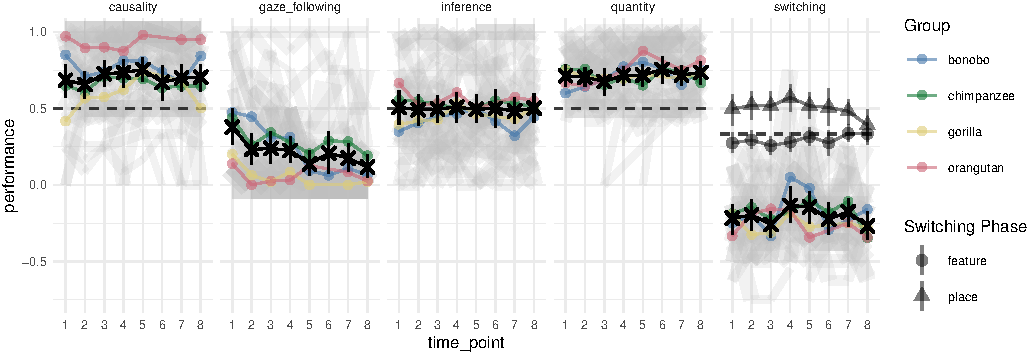
\includegraphics{figs/2-col-image-1} 

}

\caption[This image spans both columns]{This image spans both columns. And the caption text is limited to 0.8 of the width of the document.}\label{fig:2-col-image}
\end{figure*}
\end{CodeChunk}

\hypertarget{stability}{%
\subsection{Stability}\label{stability}}

First we looked at group level stability in performance. That is, we
asked how much performance varied across time points in the different
tasks. For this analysis, we ignored the temporal order of the different
time points and treated them as replications of the same experiment
(i.e.~as a factor instead of a numerical variable). As such, we asked a
meta-analytic question: how much variation is there between different
instances of the same experiment. To answer this, we fitted a mixed
model with a random intercept term for time point to the data from each
task\footnote{We modeled the trial by trial data using a binomial
  distribution in a logistic GLMM for all tasks, except switching. Here
  we modeled the score (by time point) as a truncated normal
  distribution}. As part of each model, we estimated a standard
deviation of the random intercept term (\(\tau\)), which reflects the
variation between time points.

Figure XX visualizes performance across time points. The bottom row,
gives the intercept estimate for the average effect across time points
(with 95 \% highest density interval (HDI)). For causality, inference
and quantity, we can evaluate group level performance by comparing it to
chance (50\% correct = intercept of 0 in link space). Group level
performance was reliably above chance for causality and quantity but at
chance for quantity. For gaze following, there is no such reference
level and we can simply say that at at least some individuals of all
species followed the experimenter's gaze. The switching score was
consistently negative, suggesting that - on a group level - apes did not
switch strategies.

Figure XX shows the posterior distribution of \(\tau\) for each task.
While performance was very stable for inference, quantity and switching
(\(\tau\) very close to 0), performance was slightly more variable for
causality and varied substantially for gaze following. For causality,
variation did not seem to follow a clear temporal pattern. On the other
hand, for gaze following, there seems to be a downward trend with apes
(as a group) becoming less likely to follow the experimenter's gaze. We
explore this temporal pattern in more detail below. Taken together, we
may say that 4 out of 5 measures yield stable measures of group level
performance.

\begin{CodeChunk}
\begin{figure*}[h]

{\centering 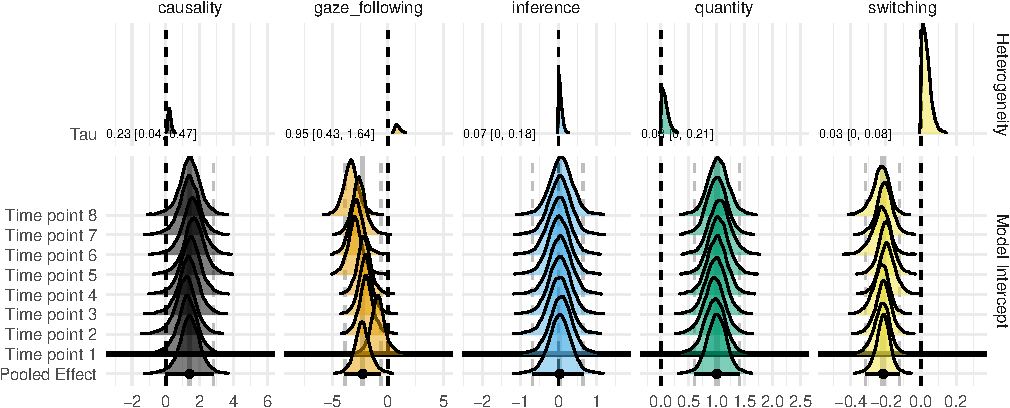
\includegraphics{figs/2-col-image3-1} 

}

\caption[This image spans both columns]{This image spans both columns. And the caption text is limited to 0.8 of the width of the document.}\label{fig:2-col-image3}
\end{figure*}
\end{CodeChunk}

\hypertarget{reliability}{%
\subsection{Reliability}\label{reliability}}

Next, we asked how stable performance is on an individual level. This
question also relates to the reliability of each task - how well suited
it is to capture differences between individuals. In general,
reliability is high if individuals are consistently ranked across
measurement instances. One way to assess reliability is to correlate
performance from two time points (re-test reliability). Because we had
multiple time points, we computed pairwise correlations for all
combinations of time points (total of 28 unique correlations per task).
This results in a distribution of correlations, which we visualize in
Figure XX. Results suggest good re-test reliability for gaze following,
causality and inference, variable reliability for quantity and poor
reliability for switching. This pattern is interesting in light of the
group level performance we reported above: stable performance on a group
level does not imply stable individual differences. We come back to this
point in the discussion.

\begin{CodeChunk}
\begin{figure}[H]

{\centering 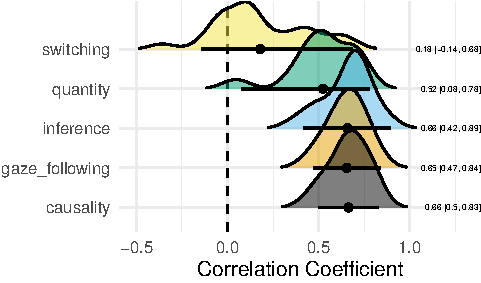
\includegraphics{figs/plot-1} 

}

\caption[R plot]{R plot}\label{fig:plot}
\end{figure}
\end{CodeChunk}

\hypertarget{predictors}{%
\subsection{Predictors}\label{predictors}}

In the final set of analysis, we investigated if variation in cognitive
performance could -- in part -- be explained by participant
characteristics. We chose to look at variables that are commonly
analyzed in the primate cognition literature: age, sex, rank and rearing
history. Rank was rated by animal keepers at every time point and
rearing history was classified as ``mother reared'', ``human reared''
and ``unknown''.

For each task, we ran the same five models\footnote{We used the same
  response distributions as in the stability analysis.}: A baseline
model predicting performance by time point (numerical) and trial as well
as four models, each with one of the predictors (age, sex, rank and
rearing history) added to the baseline model. We did not investigate any
interaction models (interactions among the predictors or with time
point) because we had no specific hypothesis in that direction. We used
Bayesian model comparison based on WAIC (widely applicable information
criterion) scores and weights {[}cite McElreath book{]}. This comparison
tells us which of the models considered makes the best out-of-sample
predictions. If the model with one predictor (e.g.~age) would be
consistently assigned the highest weight across tasks, we would conclude
that cognitive performance is best predicted by participants' age.

Figure XX gives WAIC scores and weights for each model and task. Figure
XX shows the posterior distribution of the test predictors (as well as
for time point). The baseline model was ranked highest across tasks
(first or second for all tasks), suggesting that none of the test
predictors was consistently related to performance. Within the baseline
model, the estimate for time point was close to 0 for all tasks except
gaze following, for which it was largely negative (reflecting the
downward trend we saw in Figure XX).

For gaze following, the model including sex as predictor was ranked
highest: males were somewhat less likely to follow the experimenter's
gaze. For quantity, the rank model was rated highest with lower ranking
individuals showing better quantity discrimination.

Taken togther

\begin{CodeChunk}
\begin{figure*}[h]

{\centering 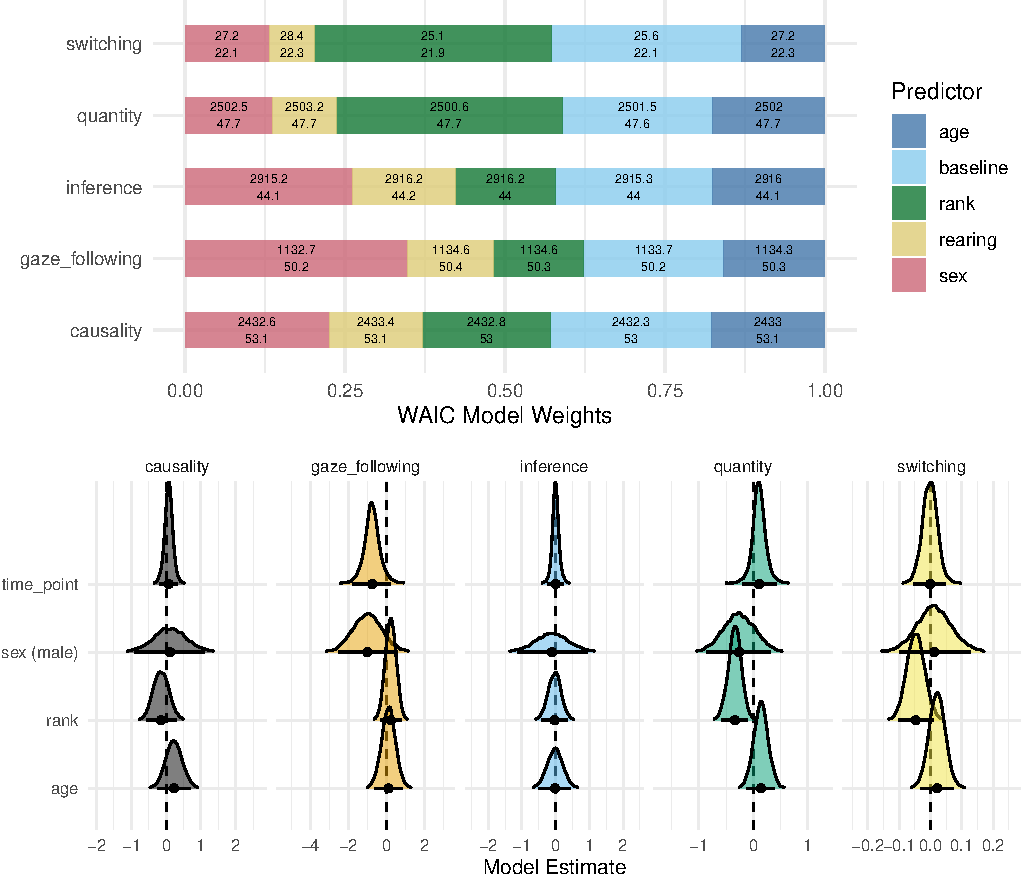
\includegraphics{figs/2-col-image2-1} 

}

\caption[This image spans both columns]{This image spans both columns. And the caption text is limited to 0.8 of the width of the document.}\label{fig:2-col-image2}
\end{figure*}
\end{CodeChunk}

\hypertarget{discussion}{%
\section{Discussion}\label{discussion}}

Reliability is independent from group level performance (leaving aside
floor and ceiling effects); thus, a task may be highly reliable even if
group level performance is at chance level {[}cite Hedge paper{]}. Here,
we see such a pattern for inference. Group level performance is
consistently at chance level for every time point. On a group level, one
would conclude that great apes do not make the inference in question.
However, the tasks is highly reliable, suggesting that accurately
captures individual differences. Together with the observation that some
individuals consistently perform at ceiling (see Figure XX), this
suggests that the task is well suited to measure inferential abilities
on a individual level. The opposite pattern holds for quantity. Here,
group level performance is consistently above chance but individual
differences are not very consistent, suggesting that variation is due to
sources other than systematic differences between individuals. This
Phenomenon is quite common in the adult cognitive literature (e.g.~Hedge
paper) and arises when experimental tasks (optimized for low variance in
measurement) are used to study individual differences (requiring high
variance in measurement). In sum, when planning to study individual
differences by relating measures to one another, researchers are well
advised to first study the reliability of these measures. Even though
this takes considerable time and effort, it increases to the chances to
find effects.

Predictors: no predictor makes sense everywhere - carefully select them
based on theoretical considerations. Avoid including them just to
control for stuff (cite paper Mike Frank mentioned:
\url{https://journals.plos.org/plosone/article?id=10.1371/journal.pone.0152719})

\hypertarget{acknowledgements}{%
\section{Acknowledgements}\label{acknowledgements}}

Place acknowledgments (including funding information) in a section at
the end of the paper.

\hypertarget{references}{%
\section{References}\label{references}}

\setlength{\parindent}{-0.1in} 
\setlength{\leftskip}{0.125in}

\noindent

\bibliographystyle{apacite}


\end{document}
